\chapter{Abordagem~\textit{JOGUE-ME}}\label{chapter:abordagem_gahme}
Para desenvolver um~\ac{sms} dos sinais motores, usando jogos eletrônicos como interface de entrada de dados (\ac{jogue-me}). É necessário analisar quais os movimentos e ações o usuário deve executar para que seja possível identificar os sinais motores, a partir das ações dos usuários. De posse dos movimentos, estes devem ser testados junto a indivíduos portadores da deficiência a ser monitorada e indivíduos como grupo de controle para avaliar a viabilidade de detecção do sinal.

%A classificação mais ampla dos tipos de jogos separa-os em jogos para entretenimento, jogos sérios (\textit{serious games}) e simuladores. Os desenvolvedores de jogos eletrônicos usam técnicas de psicologia ~\cite{sweetser2005-gameflow} para estimular e concentrar o jogador nos desafios propostos pelo jogo. Logo, os requisitos para a concepção de um jogo demandam estímulos das funções cognitivas, aquisição de novos conhecimentos além de execução de ações específicas na interação com jogos que realizam capturas de movimento ~\cite{machado2011}. Por esse motivo, é que alinhar a jogabilidade e a possibilidade de monitoramento contínuo dos dados de saúde não é uma tarefa trivial. Pois deve ser levado em consideração o uso dos dispositivos e pensar na execução de movimentos ou ações que permitam esse monitoramento.





%\subsection{Requisitos de Jogos Com o Propósito de Monitoramento de Dados Motores}
%Nessa seção serão apresentados requisitos identificados durante a análise qualitativa da Entrevista Semi-Estruturada realizada com os profissionais de saúde conforme a metodologia de pesquisa. Para uma melhor análise dos resultados as considerações identificadas durante a análise foi confrontada com as diretrizes médicas ~\cite{protpar010,Jankovic_2008,ambulatoryparkinson2010} e a revisão da literatura sobre jogos para saúde \ref{section:jogos_saude} que serviram de base científica para esse trabalho.
%
%\subsubsection{Requisitos Essenciais}
%\begin{description}
	%\item[RE-001: – Progresso do jogo]
	%\item[RE-002: 
%\end{description}

%Requisitos Essenciais
%[RE-001] – Progresso do jogo
%Segundo Suhonnen, a característica mais atrativa de um jogo é perceber o progresso do mesmo. É o usuário conseguir visualizar o progresso do jogo [8].
%[RE-002] – Estado de Fluxo ou Escapismo
%O jogador tem que sentir relaxado e com desejo de repetir a atividades em outras oportunidades [8], o jogo tem que permitir que o usuário entre num estágio de fluxo [20] e execute as atividades sem perceber a noção de tempo e espaço. O usuário deverá jogar pelo próprio prazer.
%[RE-003] – Pontuação e Taxas de Acerto
%O jogador deve visualizar suas ações positivas e negativas. O jogo deverá pontuar as atividades do jogador de acordo com seus acertos. O jogador deve visualizar claramente os objetivos e perceber o sucesso ou fracasso alcançado [8], [15].
%[RE-004] – Preocupação física do jogador
%Por promover atividades físicas, ou ações que possam trazer injúria ao jogador, como movimentos de equilíbrio, movimentos repetitivos ou rápidos. O game design do jogo deve ter a preocupação de desenvolver o jogo de acordo com o público-alvo. Isso significa dizer que a faixa etária e limitações físicas e cognitivas em decorrência da idade ou enfermidade devem ser levadas em consideração. Os jogadores devem ter a segurança de usarem o jogo e ter a certeza que o seu uso não acaarretará em nenhum dano físico [1].
%[RE-004] – Monitoramento 
%O jogo poderá monitorar os sinais vitais através dos sensores usados como interface do jogo. Sensores de movimento, podem ser aplicados para movimentar o personagem. Monitores cardíacos para controlar a intensidades dos exercícios físicos. Eletroencefalograma podem ser usados para acompanhar o nível de concentração do jogador [15]. A partir dos dados capturados, estes podem ser armazenados para uma avaliação a posteriori por um profissional de saúde. Desta maneira teremos um monitoramento dos dados de saúde de maneira não invasiva e presente na rotina do usuário.
%Requisitos Secundários
%[RS-001] – Motivar atividade física
%Os jogos para monitoramento de saúde que fazem uso de sensores de movimento, normalmente mootivam a prática de exercícicio físico [1], [8], [15]. Logo, esse requisito pode ocorrer de forma secundária sem ser o propósito principal do jogo.
%[RS-002] – Promover Reabilitação
%Para alguns tipos de usuário o jogo poderá ser usado para reabilitação. Usuários que tenham passado por acidentes vascular cerebral, cirurgia recente em algum membro. Estudos indicam que os jogos para exercício físico podem ser aplicados para auxiliar a reabilitação do usuário. Então como requisito secundário poderia atender a esse fim.
%[RS-003] – Acompanhamento ao Tratamento
%Através da abordagem do jogo será possível influenciar o jogador a uma maior aderência ao tratamento[13], [14]. Contudo essa abordagem é difícil de ser adequada para um jogo voltado ao entretenimento.


%\begin{enumerate}
%
%\item{Solução não invasiva: não ser vestida, nem invasiva fisicamente, conforto... }
%\item{Solução pervasiva: ser integrada às atividades do dia a dia... }
%\item{Ser segura em relação a integridade física: }
%\item{Ser computacionalmente viável: é possível utilizar as soluções computacionais atuais para implementar a solução}
%
%
%
%\end{enumerate}

\section{Definição de Requisitos da Solução}\label{section:requisitos_solucao}
Com base no levantamento bibliográfico e nas entrevistas semiestruturadas~\cite{FLI04} com profissionais de saúde, identificamos e enumeramos os seguintes requisitos funcionais, os quais devem ser desenvolvidos para uma solução \ac{jogue-me}:

\begin{description}
	\item[REQ-JOGUE-ME-01 - Pontuação e Taxa de Acerto]: O jogador percebe os objetivos e visualiza o sucesso ou fracasso alcançado. O jogo pontua o jogador de acordo com seus seus erros e acertos~\cite{Suhonen:2008:SFE:1457199.1457204,sinclair07}.
	\item[REQ-JOGUE-ME-02 - Progresso e Evolução do Jogador e dos Desafios]: O jogador percebe seu progresso e evolução no jogo. Os desafios tonam-se mais complexos no decorrer do tempo ~\cite{Suhonen:2008:SFE:1457199.1457204}.
	\item[REQ-JOGUE-ME-03 - Estado de Fluxo]: Um dos grandes desafios de um jogo eletrônico é levar o usuário a um ``Estado de Fluxo'' ou escapismo, passando a executar a atividade proposta pelo jogo de uma forma autotélica, ou seja, o usuário não vislumbra um benefício imediato ou futuro ~\cite{sweetser2005-gameflow}. 
	\item[REQ-JOGUE-ME-04 - Preocupação com Integridade Física do Jogador]: Promover atividades físicas ou ações que venham a trazer injúria ao jogador, como: movimentos de equilíbrio, movimentos repetitivos ou bruscos ~\cite{arntzen2011,sinclair07}.
	\item[REQ-JOGUE-ME-05 - Captura e Armazenamento de Sinais Motores]: O jogo deve realizar a captura dos sinais motores do usuário usando sensores de movimento. Os dados capturados são enviados à um servidor para tornar possível o acompanhamento da saúde motora.
	\item[REQ-JOGUE-ME-06 - Mecanismo de Identificação de Sinais Motores]: Baseados em algoritmos de aprendizagem de máquina, o servidor acompanha todos os usuários do sistema e identifica qual deles está com distúrbio motor, em caso afirmativo, envia-se a informação ao profissional de saúde.
	\item[REQ-JOGUE-ME-07 - Mecanismo de Visualização dos Parâmetros Motores do Usuário]: O profissional de saúde poderá visualizar os dados identificados pela máquina de aprendizagem, para realizar a tomada de decisão sobre o estado de saúde do usuário.
\end{description}

\section{Visão geral da solução}

A abordagem~\ac{jogue-me} faz uso de jogos eletrônicos como interface de aquisição de sinais, tornando os usuários mais motivados a fornecer seus sinais motores, em comparação ao uso dos dispositivos vestíveis. Então, com o uso da presente abordagem, um paciente portador de uma doença motora, no conforto do seu lar, poderá fornecer sinais motores de uma maneira colaborativa e não invasiva. Por outro lado, o profissional de saúde poderá visualizar os sinais motores de seus pacientes com uma frequência muito maior, em comparação as avaliações clínicas realizadas durante o período de consulta. 

\begin{figure}[!h]
     \centering
     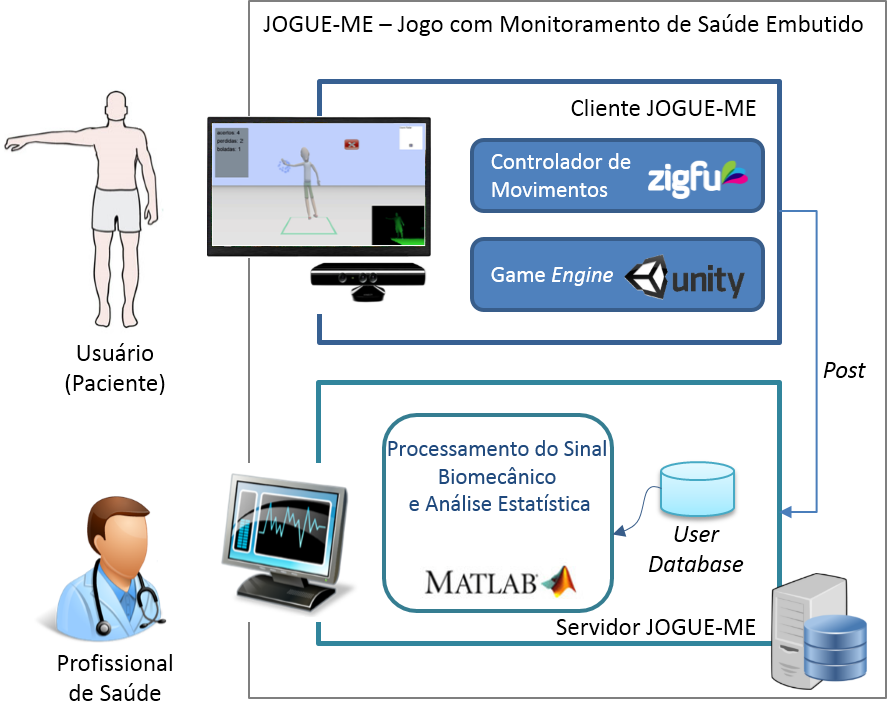
\includegraphics[width=0.78\textwidth]{./img/visaosistema.png}
     \caption{Visão Geral da Abordagem~\textit{JOGUE-ME}}
     \label{img:visaogeral}
\end{figure}

Em nosso estudo, identificamos que utilizando jogos eletrônicos como mecanismo de entrada de dados, é possível alcançar os requisitos de pervasividade e não invasividade propostos nesta tese. Pois, através dos dispositivos de sensores de movimento usados nesses ambientes, é possível desenvolver um jogo que motive o usuário a executar ações específicas, como também, possibilitem o monitoramento de sinais motores. A partir de uma interface com o usuário, que permite enviar os dados capturados a um servidor, este fará o armazenamento dos dados para um possível acompanhamento da saúde motora por um profissional de saúde.

A Visão Geral (Figura~\ref{img:visaogeral}) desta solução propõe usar técnicas de processamento de sinais para reconhecer os padrões de movimento e identificar os sinais motores. Para tornar isso factível é necessário identificar ciclos de movimento, filtrá-los e extrair características deste movimento. Após a extração das características, os dados são repassados para máquinas de aprendizagem, as quais são responsáveis por classificar os dados, baseadas em evidências estatísticas. Caso a máquina identifique algum usuário com distúrbio motor, ela poderá notificar o profissional de saúde para que este visualize os dados e tenha um melhor suporte para a tomada de decisão em relação ao tratamento.

%A abordagem \textit{GAHME} pode ser vista como uma caixa preta que recebe como entrada os dados motores de indivíduos e tem como saída técnicas de aprendizagem de máquina para identificar a ocorrência sinais motores. Caso a máquina de aprendizagem identifique algum problema motor em um indivíduo o Profissional de saúde poderá visualizar os dados e realizar a tomada de decisão sobre o tratamento.

%O Processamento de Sinais Biomecânicos e a Aprendizagem Supervisionada usam classificadores de dados. Esses módulos realizam o processamento dos dados com o objetivo de filtrar ciclos de movimento que possibilitem a identificação de sinais de motores de saúde e como consequência possam extrair as características desse movimento. Após a extração das características, os dados são repassados para Máquinas de Aprendizagem que classificam os dados por intermédio das evidências estatísticas encontradas neles como iremos explicar no decorrer deste capítulo.

O funcionamento da abordagem pode ser descrito como uma composição de quatro passos: captura dos sinais através de sensores, processamento de sinais biomecânicos, classificação dos dados e visualização.

\section{Aquisição de Dados}
O propósito de um \ac{jogue-me} é coletar informações do estado motor dos indivíduos de forma não invasiva. Por este motivo, foi apresentada uma abordagem de jogos eletrônicos como infraestrutura de aquisição de sinais motores, por meio dos sensores de movimento utilizados em jogos eletrônicos.

O cliente \ac{jogue-me} é um jogo com funcionalidades de aquisição de dados motores de movimentos específicos. Logo, ele realiza a captura e envio de dados para um servidor, que recebe requisições para efetuar o recebimento e armazenamento das informações, o que torna possível: armazenar o histórico do usuário para um acompanhamento dos sinais motores por um longo período. Desta maneira, um profissional de saúde poderá visualizar a evolução da saúde motora do usuário.

\section{Processamento de Dados Biomecânicos}\label{sec:processador_bio}
O módulo de Processamento de Dados Biomecânicos é responsável por: filtrar, remover ruídos e identificar ciclos de movimento para uma posterior extração dos vetores de características, como pode ser visto na Figura~\ref{img:process_bio}. A partir dos sinais processados, aplicam-se técnicas de aprendizagem de máquina para obter a classificação dos sinais e, consequentemente, validar este trabalho.

\begin{figure}[!htb]
     \centering
     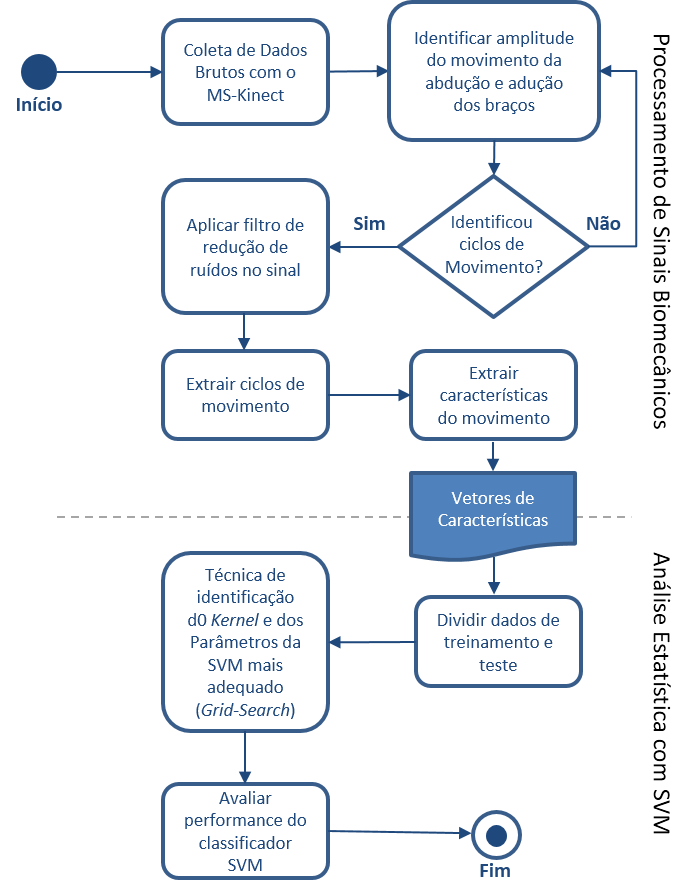
\includegraphics[width=0.8\textwidth]{./img/biomecprocessor2.png}
     \caption{Processamento de sinais biomecânicos.}
     \label{img:process_bio}
\end{figure}


\subsection{Identificação de Ciclos de Movimento}\label{section:identificao_ciclos}

Os sinais adquiridos por sensores de movimento possuem bastante ruído, o que dificulta a identificação dos ciclos de movimento, pois eles possuem uma posição que inicia o ciclo de movimento, como na Figura~\ref{img:exsinalposicaopunho}, e o ruído existente pode cruzar por essa linha e, consequentemente gerar falsas identificações. 

%Métodos que fazem uso de filtros podem ser aplicados para suavizar a curva e diminuir a ocorrência do ruído, contudo, isso implica numa alteração no tempo do sinal o que impacta diretamente no cálculo das características do movimento e, como consequência na acurácia do resultado final~\cite{peakdetect}.

\begin{figure}[!htb]
     \centering
     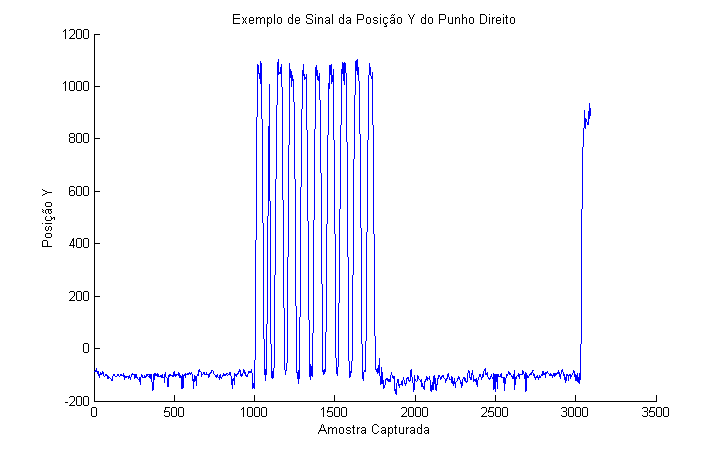
\includegraphics[width=1\textwidth]{./img/exsinalposicaoypunhodireito.png}
     \caption{Exemplo de Sinal Capturado da Articulação do Punho do Direito Usando MS-Kinnect na Posição Y}
     \label{img:exsinalposicaopunho}
\end{figure}

Em casos de análise de sinais biomecânicos da amplitude do movimento, é possível aplicar a técnica de detecção de picos e vales do sinal~\cite{peakdetect}. Esta técnica consiste em usar um valor de referência, $\delta$\ (\textit{delta}), para identificação dos picos e descartar valores menores que são considerados ruídos. O pico é o ponto mais alto entre os 2 pontos mais baixos, que são considerados os vales do ciclo. A técnica é aplicada no sinal da Figura~\ref{img:exsinalposicaopunho}, com um $\delta$\ de 500 e teve como resultado os picos e os vales identificados como pode ser visto na Figura~\ref{img:expicosvales}.

\begin{figure}[!htb]
     \centering
     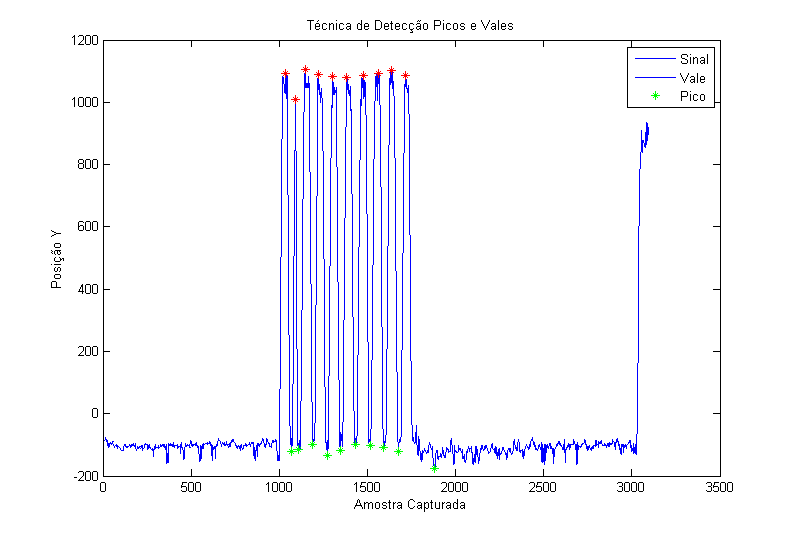
\includegraphics[width=1\textwidth]{./img/deteccaopicosvales.png}
     \caption{Exemplo da Aplicação da Técnica de Detecção de Picos e Vales no Sinal}
     \label{img:expicosvales}
\end{figure}


%\subsubsection{Redução de Ruídos no Sinal}
O processo de Identificação de Ciclos de Movimento é realizado em 3 etapas distintas:
\begin{itemize}
	\item Identificar ciclos de movimentos;
	\item calcular movimento angular realizado durante o ciclo de movimento;
	\item remover ciclos de movimentos incompletos.
\end{itemize}

Para identificar os ciclos de movimento de adução e abdução dos braços, é necessário utilizar uma das articulações como referência. Neste movimento, a articulação do punho (Figura~\ref{img:remocaoruidossinal}) é a que possui o sinal como maior amplitude entre as demais, por esse motivo, esta é a escolhida para identificar os ciclos. Realiza-se a técnica de picos e vales no sinal do \textit{punho} para identificar o início e o fim do movimento de adução e abdução dos braços. Depois de identificado onde começa e termina o movimento, calcula-se o deslocamento angular através do produto escalar entre as articulações do punho, ombro e bacia(Seção~\ref{section:movimento_abducao}). Neste momento, o sinal irá conter ciclos de movimentos angulares, realiza-se uma nova eliminação de ruídos, ao extrair os ciclos de movimento identificados no sinal. Essa é a primeira etapa da filtragem dos dados, a qual seleciona o início e o fim dos ciclos de movimentos. Depois desta etapa, realiza-se a extração de cada ciclo e 
identifica sua 
completude, para que as características extraídas dos ciclos de movimento sejam semelhantes para cada indivíduo e torne possível a classificação dos dados.

\begin{figure}[!htb]
     \centering
     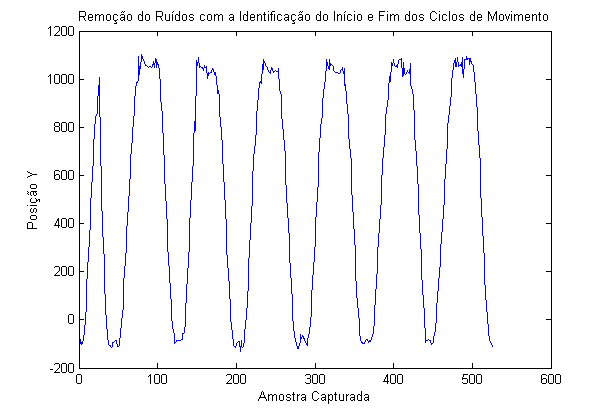
\includegraphics[width=1\textwidth]{./img/remocaoruidociclo.png}
     \caption{Remoção de Ruídos}
     \label{img:remocaoruidossinal}
\end{figure}


\subsection{Extração das Características do Movimento} \label{sec:extracao_caracteristcas}
As características do sinal a ser obtido é baseada na cinemática do movimento angular. Logo, é necessário um estudo da biomecânica do movimento humano nos ciclos de movimento ~\cite{hamill1999bases}. De posse do tempo de ocorrência de cada ciclo e das articulações do \textbf{punho}, \textbf{bacia} e \textbf{ombro}. Deve-se calcular o ângulo relativo do movimento de abdução e adução do braço através da aplicação do teorema do produto escalar, que encontra o ângulo entre dois vetores dentro do intervalo de $0 \leq \theta \leq 180º$.

\subsubsection{Cálculo do Ângulo Relativo do Movimento de Abdução e Adução}\label{section:movimento_abducao}
O produto escalar é uma operação entre dois vetores cujo resultado é um escalar~\cite{algebra90}. Então, o ângulo entre dois vetores é definido como ``o menor'' ângulo entre eles. Desta forma, este ângulo está dentro do intervalo de $0 \leq \theta \leq 180º $. O produto escalar é o ângulo de $ \theta$ formado entre os vetores $ v $ e $ w $.


% \begin{equation}
% cos(\theta) = (v . w) /  (||v|| ||w||) 
% \label{eq:produto_escalar}
% \end{equation}
% 
% 
% \begin{figure}[!htb]c
%      \centering
%      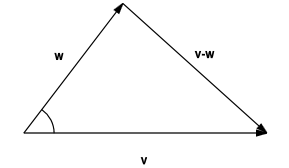
\includegraphics[width=0.5\textwidth]{./img/produtoescalar.png}
%      \caption{Produto Escalar Entre 2 Vetores}
%      \label{img:produto_escalar}
% \end{figure}

No movimento de abdução e adução do braço (Figura \ref{fig:movabducaoaducao}), o ângulo relativo pode ser calculado com as Posições ($ x $\ ,  $ y $\ , $ z $\ ) das articulações (\textit{quadril}, \textit{ombro} e \textit{punho}) utilizando o produto escalar entre esses pontos, onde extrai as características do movimento, como amplitude do movimento e, quando relacionamos com o tempo, conseguimos extrair a velocidade angular deste movimento. Como pode ser o sinal, em °/ms visto na Figura~\ref{img:amplitude_braco}, quantificando, o movimento da adução e abdução do braço em relação ao tempo.

%O ângulo relativo podem ser calculados usando a Lei dos Cossenos. Essa lei é simplesmente um caso mais geral do Teorema de Pitágoras e descreve a relação entre os lados de um triângulo. Para nossos propósitos, o triângulo é constituído por dois segmentos (b e c) e uma linha (a) unindo a ponta distai de um segmento com a ponta proximal do outro ~\cite{hamill1999bases}.

\begin{figure}[!htb]
     \centering
     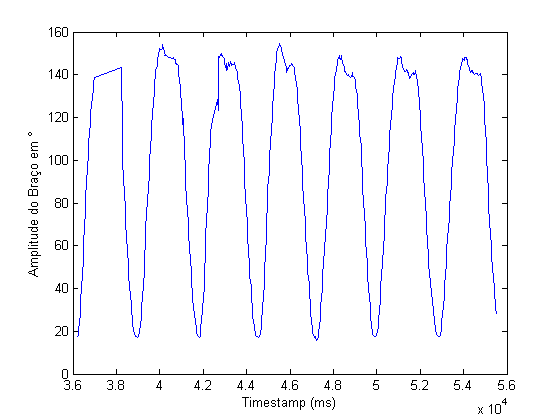
\includegraphics[width=1\textwidth]{./img/amplitude-braco.png}
     \caption{Amplitude do Movimento de Abdução e Adução}
     \label{img:amplitude_braco}
\end{figure}


% \lstset{language=Matlab}          % Set your language (you can change the language for each code-block optionally)
% \begin{lstlisting}[frame=single, caption=Código do Ângulo Relativo por Produto Escalar, label=code:produto_escalar]  % Start your code-block
% Bacia = [articulacaoBacia(PosicaoX), articulacaoBacia(PosicaoY), articulacaoBacia(Posicaoz)];
% Ombro = [articulacaoOmbro(PosicaoX), articulacaoOmbro(PosicaoY), articulacaoOmbro(Posicaoz)];
% Punho = [articulacaoPunho(PosicaoX), articulacaoPunho(PosicaoY), articulacaoPunho(Posicaoz)];
% 
% w = Bacia-Ombro;
% v = Punho-Ombro;
% 
% CosTheta = dot(w,v)/(norm(w)*norm(v));
% ThetaEmGraus = acos(CosTheta)*180/pi;
% \end{lstlisting}

\subsubsection{Cálculo da Velocidade Angular do Movimento de Abdução e Adução}
O pico da amplitude do movimento irá conter a amplitude máxima desse movimento. O tempo gasto entre 1° vale até o pico em cada ciclo de movimento, será o tempo gasto para a abdução do braço e, o tempo gasto entre o pico e o 2° vale de cada ciclo, será o tempo gasto para a adução do braço. Portanto, com a amplitude máxima e o tempo gasto nesses movimentos, podem ser calculadas as velocidades angulares de abdução e adução dos braços, como na Figura~\ref{img:amplitude_braco_picos_vales}.
\begin{figure}[!htb]
     \centering
     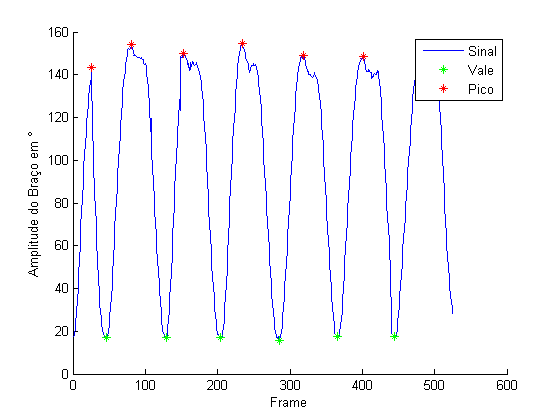
\includegraphics[width=1\textwidth]{./img/amplitude-braco-picos.png}
     \caption{Detecção de Picos e Vales da Amplitude do Movimento de Abdução e Adução do Braço}
     \label{img:amplitude_braco_picos_vales}
\end{figure}

\subsection{Filtragem de Dados}\label{section:filtro_dados}

A filtragem dos dados consiste na realização das seguintes etapas nos ciclos de movimento:
\begin{description}
	\item [Escalonar os ciclos]: O conjunto de dados deve possuir a distribuição de \textbf{M} amostras de vetores de dimensão \textbf{n}. Como os dados a serem analisados são sinais, deve-se então escalonar o sinal para uma dimensão \textbf{n} para poder realizar o cálculo matricial quadrático de (\textbf{M} x \textbf{n}).		
	\item [Normalizar os ciclos]: Em estatística, o termo normalização possui diferentes significados ~\cite{statisticterms2006}. Neste trabalho, a normalização consiste no ajuste dos valores dos dados em torno do valor máximo. Ou seja, o máximo valor obtido dos dados terá o valor 1 e, os demais, será o resultado pela divisão do valor máximo. A normalização se faz necessária para que a variação dos dados seja mantida, além de facilitar a identificação de similaridades ~\cite{vicini2005}. 	
	\item [Calcular Vetor Médio dos Ciclos]: Para definir a completude de um ciclo de movimento, deve-se, calcular a média entre todos os ciclos de movimento, que é o vetor médio dos ciclos escalonados e normalizados (Figura ~\ref{img:ciclos_normalizado_escalonado}). O \textbf{vetor médio}, Equação (\ref{eq:vetormedio}), chamado de $\bar{X}$\, consiste na média aritmética de todos os ciclos de movimento, ou seja, calcula a centralização dos dados ~\cite{statisticshandbook2009}. 	
		\begin{equation}
			\bar{X}=\frac{\sum_{i=1}^{n}(Xi)}{(n)}
			\label{eq:vetormedio}
		\end{equation}
	\item [Calcular Variância de Cada Ciclo ao Vetor Médio]: A variância é uma medida de dispersão estatística, que indica o quão longe os estão de um valor esperado~\cite{statisticshandbook2009}. Neste caso, o valor esperado é o vetor médio dos ciclos ($\bar{X}$), e a variância, Equação (~\ref{eq:variancia}), irá nos informar o quão distante cada ciclo ($C$) está em relação a média.
		\begin{equation}
			var(C) = (C - \bar{X} )^2
			\label{eq:variancia}
		\end{equation}
		
		
	\item [Definir limiar para remoção de ciclos]: Essa etapa do processo de filtragem não é trivial, pois deve-se definir uma constante, $ filtro $\, que será comparada à variância do ciclo, se esta for menor, será aceita, caso contrário, removida. Contudo, balancear entre o limiar de dispersão do ciclo de movimento em relação a média é complexo, pois existe uma grande variabilidade de movimento. Logo, um limiar muito alto pode acarretar na remoção de uma grande quantidade de ciclos. Por outro lado, um limiar baixo colocaria ruídos nos dados e consequentemente impactaria no resultado da classificação.	
	\lstset{language=Matlab}
	\begin{lstlisting}[frame=single, caption=Filtro dos Ciclos]  % Start your code-block
		
    filtro = 1;
    vetorMedio = mean(ciclos);
    varianciaCiclo = sum(ciclo - (vetorMedio).^2);
    remocao = varianciaCiclo>filtro;
	\end{lstlisting}
	
	\begin{figure}
     \centering
     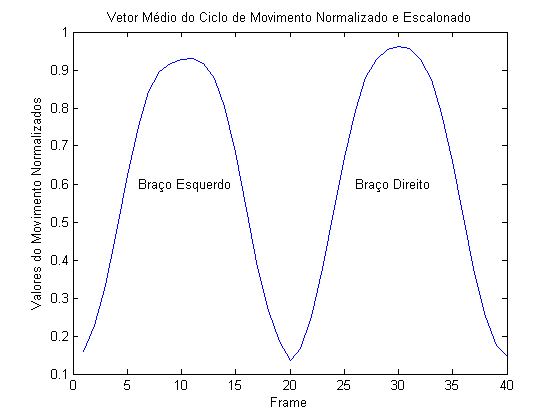
\includegraphics[width=1\textwidth]{./img/vetormedionormalozadoescalonado.png}
     \caption{Ciclos de Movimento Normalizados e Escalonados}
		 \label{img:ciclos_normalizado_escalonado}
	\end{figure}
\end{description}


%\lstset{language=Matlab}
%\begin{lstlisting}
	%normalizarCiclos(ciclos);
	%escalonarCiclos(ciclos, CONSTANTE_ESCALONAMENTO);
	%vetormedio = mean(ciclos);
	%
	%
%\end{lstlisting}

%%Média

Como exemplo, temos um ciclo de movimento filtrado (Figura~\ref{img:ciclo_filtrado}) (\textit{valor do filtro = 1}) e o (\textit{valor da variância = 2,3078}).

\begin{figure}[!htb]
     \centering
     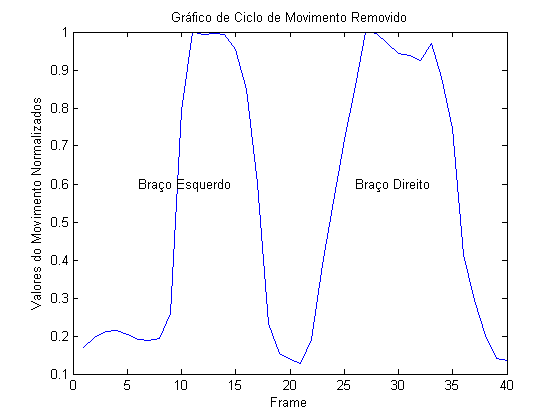
\includegraphics[width=1\textwidth]{./img/ciclomovimentoremovido.png}
     \caption{Ciclo de Movimento Removido}
		 \label{img:ciclo_filtrado}
\end{figure}


\section{Classificação de Dados por Máquina de Aprendizagem}\label{section:class_dados}
O objetivo de todo esse processo de identificação de ciclos, extração de características e filtragem, é justamente facilitar a separação dos dados por máquinas de aprendizagem. A normalização dos ciclos, ficou como o resultado do cálculo do produto escalar que nos retorna valores entre $ 0° $\ a $ 180° $\, do movimento de abdução e adução. O escalonamento de cada ciclo de movimento ficou com 20 \textit{frames}, como temos o movimento do braço esquerdo e depois o do direito, temos um total de 40 \textit{frames} por ciclo. O motivo pelo qual decidimos juntar os ciclos do braço esquerdo, direito, lado a lado, foi justamente para facilitar a identificação da assimetria do movimento existente nos estágios iniciais da ~\ac{dp}. Portanto, o classificador será responsável por identificar os indivíduos diagnosticados com~\ac{dp}, por meio das diferenças de movimento existente entre estes e os indivíduos sem o diagnóstico da doença. 

O vetor de características é composto dos ciclos de movimento e das características extraídas de cada ciclo, conforme explicado na Seção~\ref{sec:extracao_caracteristcas}. Ou seja, terá, além do ciclo de movimento, os valores da velocidade angular de abdução e adução do braço esquerdo e direito. De posse desse vetor de características e do rótulo sobre a classe do ciclo de movimento (indivíduo diagnosticado com~\ac{dp} e indivíduo sem o diagnóstico estabelecido), esses dados serão repassados como entrada-saída para o classificador de dados, que irá dividir entre grupos de treinamento e teste para realizar sua classificação.

Nesta abordagem, o classificador de dados será usado para identificar usuários com problemas motores. Desta forma, irá auxiliar o profissional de saúde no acompanhamento de seus pacientes. Supondo que um profissional de saúde detém um grande número de pacientes, e que estes fazem uso da abordagem~\ac{jogue-me} para monitorar seus dados, caso fosse identificado algum sinal motor, o profissional de saúde seria notificado e poderia visualizar as informações que auxiliam a tomada de decisão.





\section{Visualização dos Dados}
O acompanhamento dos sinais motores é necessário, principalmente, para doenças crônicas de impacto motor e que tenham melhoria nos sinais. Pois assim, auxilia o médico no acompanhamento motor e, consequentemente, permite tratar o paciente de acordo com a resposta ao tratamento.

Como exemplo da abordagem, o profissional de saúde poderia visualizar as características dos movimentos, que serviram como dados de entrada para a máquina de aprendizagem. Nesse caso, podemos ver duas tabelas em que é possível identificar as diferenças motoras de uma pessoa diagnostica com a ~\ac{dp} (Tabela~\ref{table:extracao-caracteristica}) e um indivíduo sem o diagnóstico da doença (Tabela~\ref{table:extracao_caracterisca_saudavel}).

\begin{table}[h]
\begin{tabular}{|r|r|r|r|r|r|}
\hline
\multicolumn{4}{|l}{Velocidades º/S}                                                                                                                                                                                                                                                                                         & \multicolumn{2}{|l|}{Amplitudes}     \\ \hline
\multicolumn{1}{|l}{\textbf{\begin{tabular}[c]{@{}c@{}}Abdução\\ Esquerda\end{tabular}}} & \multicolumn{1}{|l|}{\textbf{\begin{tabular}[c]{@{}c@{}}Abdução\\ Direita\end{tabular}}} & \textbf{\begin{tabular}[c]{@{}c@{}}Adução\\ Esquerda\end{tabular}} & \textbf{\begin{tabular}[c]{@{}c@{}}Adução\\ Direita\end{tabular}} & \textbf{Esquerda} & \textbf{Direita} \\ \hline
78,95                                                                                    & 77,82                                                                                    & 83,06                                                              & 106,42                                                            & 130,00            & 124,72           \\ \hline
79,94                                                                                    & 34,68                                                                                    & 104,69                                                             & 39,98                                                             & 131,50            & 132,44           \\ \hline
81,05                                                                                    & 47,05                                                                                    & 107.38                                                             & 56,52                                                             & 132,22            & 123,66           \\ \hline
74,73                                                                                    & 47,09                                                                                    & 109,05                                                             & 47,75                                                             & 132,33            & 122,20           \\ \hline
72,01                                                                                    & 56,02                                                                                    & 102,36                                                             & 76,00                                                             & 131,40            & 119.75      \\ \hline
\end{tabular}
\caption{Extração das Características de Indivíduo Com Diagnóstico da ~\ac{dp}}
\label{table:extracao-caracteristica}
\end{table}

\begin{table}[h]
\begin{tabular}{|r|r|r|r|r|r|}
\hline
\multicolumn{4}{|l}{Velocidades º/S}                                                                                                                                                                                                                                                                                         & \multicolumn{2}{|l|}{Amplitudes}       \\ \hline
\multicolumn{1}{|l}{\textbf{\begin{tabular}[c]{@{}c@{}}Abdução\\ Esquerda\end{tabular}}} & \multicolumn{1}{|l|}{\textbf{\begin{tabular}[c]{@{}c@{}}Abdução\\ Direita\end{tabular}}} & \textbf{\begin{tabular}[c]{@{}c@{}}Adução\\ Esquerda\end{tabular}} & \textbf{\begin{tabular}[c]{@{}c@{}}Adução\\ Direita\end{tabular}} & \textbf{Esquerda} & \textbf{Amplitude} \\ \hline
129,35                                                                                   & 61,59                                                                                    & 78,74                                                              & 176,30                                                            & 159,39            & 143,50             \\ \hline
115,67                                                                                   & 118,15                                                                                   & 71,72                                                              & 79.46                                                             & 156,37            & 153,97             \\ \hline
120.96                                                                                   & 135,27                                                                                   & 66,70                                                              & 78,17                                                             & 154,30            & 149,91             \\ \hline
125.96                                                                                   & 137,43                                                                                   & 64,75                                                              & 81,57                                                             & 153,18            & 154,58             \\ \hline
139.99                                                                                   & 117,60                                                                                   & 69,96                                                              & 84,08                                                             & 151,68            & 148,90             \\ \hline
120,51                                                                                   & 111,92                                                                                   & 75,85                                                              & 75,18                                                             & 152,58            & 148,35             \\ \hline
\end{tabular}
\caption{Extração das Características de Indivíduo Sem Diagnóstico da ~\ac{dp}}
\label{table:extracao_caracterisca_saudavel}
\end{table}

Como pode ser visto nesses dados, a amplitude de um indivíduo diagnosticado com~\ac{dp} esta bem menor do que em um indivíduo sem o diagnóstico estabelecido. Um valor importante também pode ser identificado na velocidade de adução esquerda do indivíduo com~\ac{dp}, possui uma velocidade muito maior do que o indivíduo sem o diagnóstico. Possivelmente, porque um paciente com~\ac{dp} perde um pouco o controle sobre o membro, fazendo-o descer abruptamente~\cite{protpar010}. Desta maneira, a abordagem pretende auxiliar o profissional de saúde com o fornecimento dessa informação, para que este efetue o acompanhamento e perceba a evolução do quadro clínico do paciente. 

%O produto escalar é uma operação entre dois vetores cujo resultado é um escalar e pode ser descrito na forma:
%$ u.v = |u| |v| cos(\theta) $\ onde $ \theta $\ é o ângulo formado entre $ u $\ e $ v $\ dentro do intervalo de $0 \leq \theta \leq 180º $\.

%Se
%\begin{math}
%v.w = \left \| v \right \|\left \| w \right \|\cos \theta
%\end{math}
%, onde $ \theta $\ é o ângulo entre esses vetores. Então o \textbf{ângulo} entre dois vetores é definido como o menor ângulo entre eles.
%
%Portanto, o ângulo dentro do intervalo de $0 \leq \theta \leq 180º $\ será o resultado do produto interno
%\newline
%\begin{math} \cos \theta = (v.w)/(\left \| v \right \| \left \| w \right \|)\end{math} .

%\subsubsection{Pontos Utilizados no \textit{Ms-Kinnect} Para o Cálculo do Produto Escalar}
%A descrição da posição de um segmento ou movimento articular é tipicamente expressa com relação a uma posição inicial designada. A posição anatômica é uma referência padronizada usada por muitos anos por anatomistas, biomecânicos e médicos ~\cite{hamill1999bases}.



%\begin{figure}
 %\centering
 %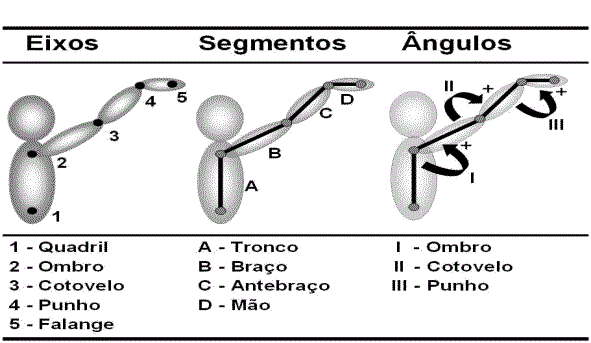
\includegraphics[scale=0.5]{./img/eixossegmentos.png}
 %% matrixargseg.png: 296x162 pixel, 100dpi, 7.52x4.11 cm, bb=0 0 213 117
 %%\caption{Estágio desenvolvimento de jogos ~\cite{fullerton2008game}}
%\caption{Eixos Segmentos e Ângulos da Biomecânica}
%%  \caption{Estágio desenvolvimento de jogos}
 %\label{fig:eixossegmentos}
%\end{figure}
